\documentclass{article}
\usepackage[utf8]{inputenc}
\usepackage[english]{babel}
\usepackage{graphicx}
%\usepackage[font=it]{caption}
\usepackage[textfont=it]{caption}

\usepackage[en-US]{datetime2}
\usepackage{minted}
\usemintedstyle{solarizedlight}

\usepackage{hyperref}
\usepackage{cleveref}

\title{Milestone 1 Evaluation\\
{\small CSE 232B, UC San Diego, Spring Q 2015}}
\author{Jens Emil Gydesen\thanks{UCSD SID: Ublah} \and
        Martin Bjeldbak Madsen\thanks{UCSD SID: U6616356}}
\date{\DTMdisplaydate{2015}{5}{13}{3}, \DTMdisplaytime{11}{10}{00}}

\begin{document}
\maketitle

Below is our brief report of milestone 1, where we had to implement a simple XQuery engine.

The repository for this project can be found here: \url{https://github.com/martinbmadsen/xquery-processor}. Although, while the quarter is active, this repository is kept private.

\section{Query 1}
Finds act, scene and speaker of famous line \emph{Et tu, Brute! Then fall, Caesar}. Should return 


\subsection{Query}\label{sec:query1query}
We modified this query slightly. First, according to the class XPath/XQuery language syntax and semantic notes\footnote{\url{http://db.ucsd.edu/cse232b/notes/xpath-semantics.pdf}}, documents are loaded with the \texttt{doc} syntax. Furthermore, we have modified \texttt{title} to \texttt{TITLE}, since XML is case-sensitive, querying on \texttt{title} would not return any valid results.

\begin{listing}[H]
\begin{minted}{xquery}
<result>{
for $a  in doc("j_caesar.xml")//ACT,
    $sc in $a//SCENE,
    $sp in $sc/SPEECH
where $sp/LINE/text() = "Et tu, Brute! Then fall, Caesar."
return <who>{$sp/SPEAKER/text()}</who>,
       <when>{<act>{$a/TITLE/text()}</act>,
             <scene>{$sc/TITLE/text()}</scene>}
       </when>
}</result>
\end{minted}
\caption{The first query.}\label{lst:query1}
\end{listing}

\subsection{Parse Tree}
\begin{figure}[H]
  \centering
  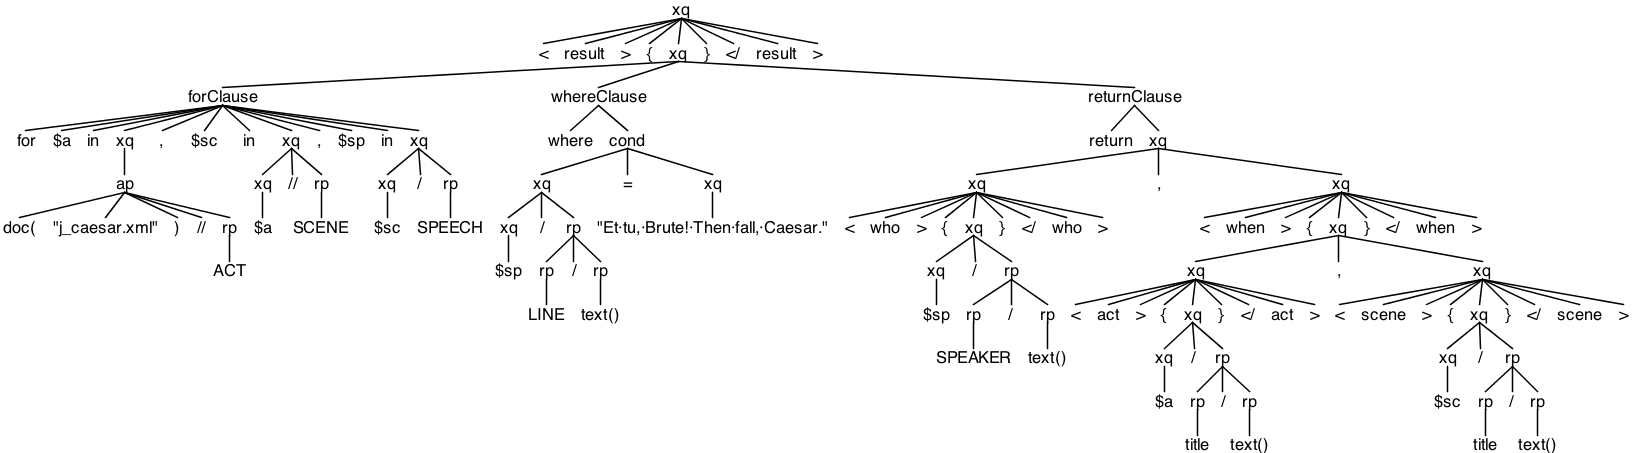
\includegraphics[width=\linewidth]{imgs/antlr4_parse_tree_query_1.png}
  \caption{Parse tree for the first query.}\label{fig:parseTree1}
\end{figure}

\subsection{Output}
\begin{listing}[H]
\begin{minted}{xml}
<result>
  <who>CAESAR</who>
  <when>
    <act>ACT III</act>
    <scene>
      SCENE I.  Rome. Before the Capitol; the Senate sitting above.
    </scene>
  </when>
</result>
\end{minted}
\caption{Output from executing query 1.}\label{lst:res1}
\end{listing}

\section{Query 2}
Groups all acts by speaker, that is, return a list of elements of type element  \texttt{speaks \{ element who \{String\}, (element when \{String\})+ \}}, where the String contents of the \texttt{<who>} element is a speaker name, and the contents of the \texttt{<when>} elements are act names.

\subsection{Query}
Again, we have modified this query a little as per the comments in \cref{sec:query1query}.

\begin{listing}[H]
\begin{minted}{xquery}
for $s in doc("j_caesar.xml")//SPEAKER
return <speaks>{<who>{$s/text()}</who>,
                for $a in doc("j_caesar.xml")//ACT
                where some $s1 in $a//SPEAKER satisfies $s1 eq $s
                return <when>{$a/TITLE/text()}</when>}
       </speaks>
\end{minted}
\caption{The second query.}\label{lst:query2}
\end{listing}

\subsection{Parse Tree}
\begin{figure}[H]
  \centering
  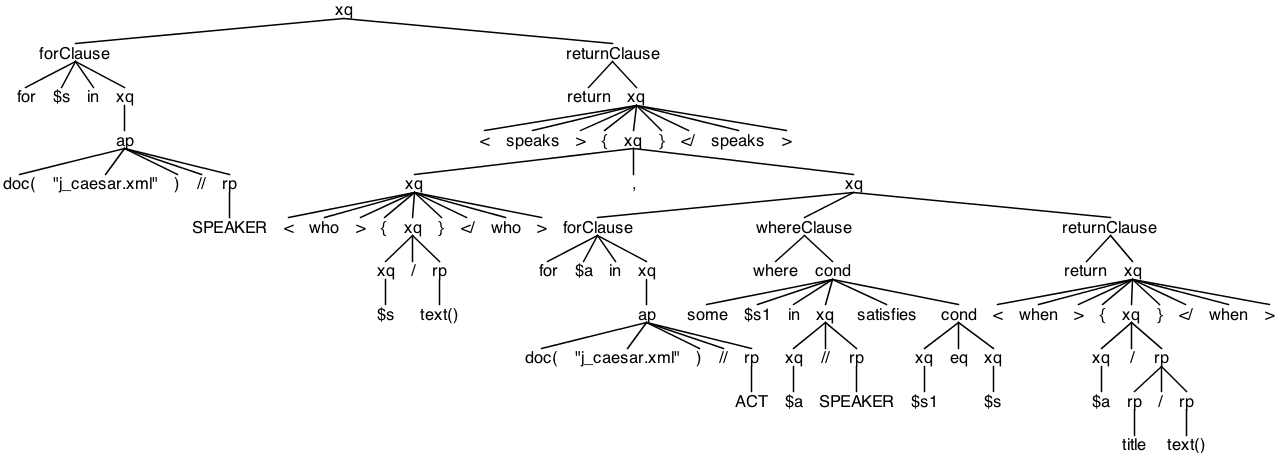
\includegraphics[width=\linewidth]{imgs/antlr4_parse_tree_query_2.png}
  \caption{Parse tree for the second query.}\label{fig:parseTree2}
\end{figure}

\subsection{Output}
\begin{listing}[H]
\inputminted{xml}{src/query2.xml}
\caption{Output from executing query 2.}\label{lst:res2}
\end{listing}

\section{Query 3}
\subsection{Query}

\begin{listing}[H]
\begin{minted}{xquery}
for $s in doc("j_caesar.xml")//SCENE
return
<scenes>{
<scene>{$s/TITLE/text()}</scene>,
for $a in doc("j_caesar.xml")//ACT
where some $s1 in $a//SCENE satisfies $s1 eq $s and $a/TITLE/text() = "ACT II"
return <act>{$a/TITLE/text()}</act>
}
</scenes>
\end{minted}
\caption{The third query.}\label{lst:query3}
\end{listing}

\subsection{Parse Tree}
\begin{figure}[H]
  \centering
  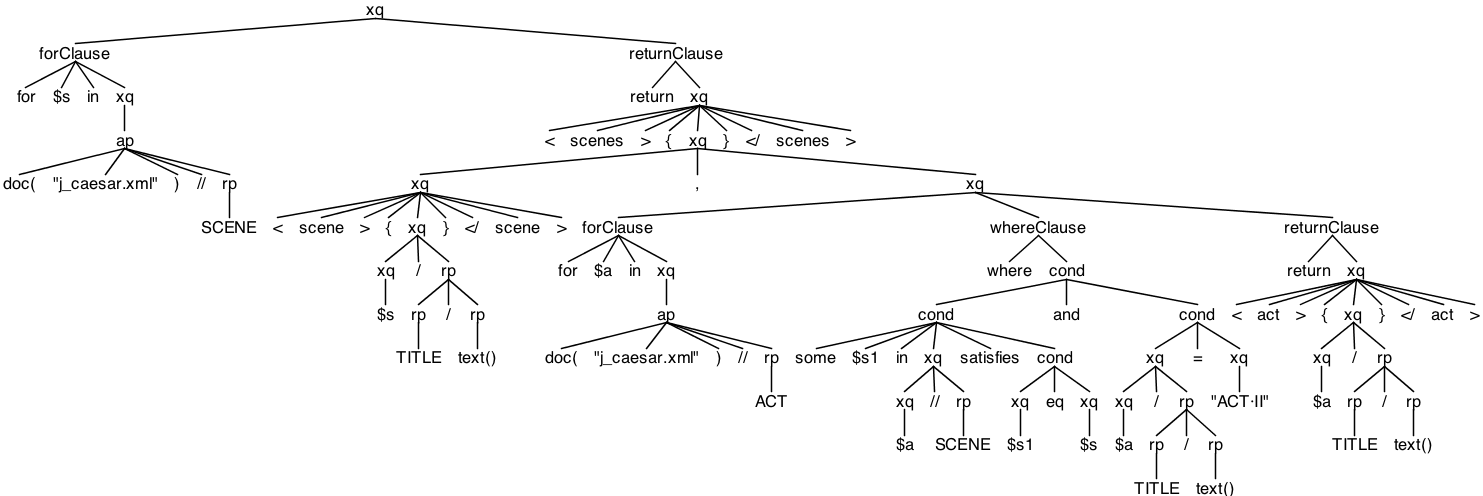
\includegraphics[width=\linewidth]{imgs/antlr4_parse_tree_query_3.png}
  \caption{Parse tree for the third query.}\label{fig:parseTree3}
\end{figure}

\subsection{Output}
\begin{listing}[H]
\inputminted{xml}{src/query3.xml}
\caption{Output from executing query 3.}\label{lst:res3}
\end{listing}

\section{Query 4}

\subsection{Query}
\begin{listing}[H]
  \begin{minted}{xquery}
    <acts> {
for $a in doc("j_caesar.xml")//ACT
where empty(
for $sp in $a/SCENE/SPEECH/SPEAKER
where $sp/text() = "CASCA”
return <speaker>{$sp/text()}</speaker>
)
return <act>{$a/TITLE/text()}</act>
}</acts>
  \end{minted}
  \caption{The fourth query.}\label{lst:query4}
\end{listing}

\subsection{Parse Tree}
\begin{figure}[H]
  \centering
  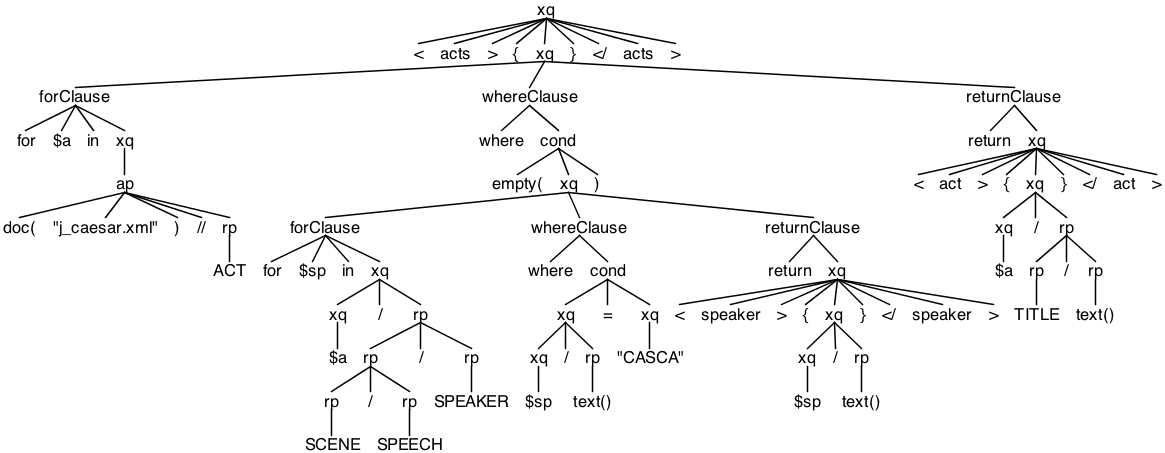
\includegraphics[width=\linewidth]{imgs/antlr4_parse_tree_query_4.png}
  \caption{Parse tree for the fourth query.}\label{fig:parseTree4}
\end{figure}

\subsection{Output}
\begin{listing}[H]
\begin{minted}{xml}
<acts>
  <act>ACT IV</act>
  <act>ACT V</act>
</acts>
\end{minted}
\caption{Output from executing query 4.}\label{lst:res4}
\end{listing}

\end{document}
